\chapter*{Appendix}
\addcontentsline{toc}{chapter}{Appendix}
\section*{List of appendices}
\vspace{-8em}

% vor \listofanhang müssen Einrückungen angepasst werden
\abstaendeanhangverzeichnis

\listofanhang
\clearpage
\spezialkopfzeile{Attachment} % damit in der Kopfzeile das Wort "Anhang" angezeigt wird

\lstset{language=TeX, % hervorzuhebende Keywords definieren
  morekeywords={anhang, anhangteil}
}

\definecolor{dkgreen}{rgb}{0,0.6,0}
\definecolor{gray}{rgb}{0.5,0.5,0.5}
\definecolor{mauve}{rgb}{0.58,0,0.82}

\lstset{frame=tb,
  language=Python,
  aboveskip=3mm,
  belowskip=3mm,
  showstringspaces=false,
  columns=flexible,
  basicstyle={\small\ttfamily},
  numbers=none,
  numberstyle=\tiny\color{gray},
  keywordstyle=\color{blue},
  commentstyle=\color{dkgreen},
  stringstyle=\color{mauve},
  breaklines=true,
  breakatwhitespace=true,
  tabsize=3,
  morecomment=[l]{\#} % This line tells 'listings' that '#' introduces a single-line comment
}

\anhang{House of Prototyping Guidelines: Prototyping Dimensions}\label{attachement:prototyping_dimensions}
\begin{figure}[htb]
\centering
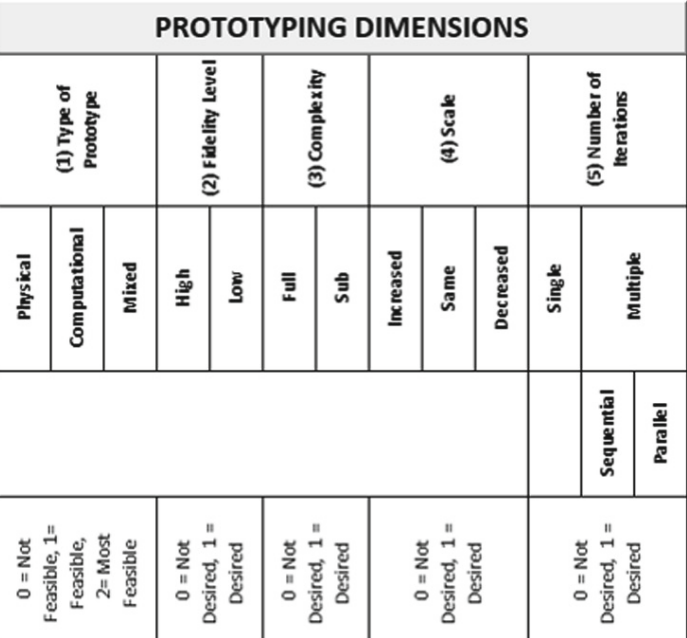
\includegraphics[width=0.9\linewidth]{graphics/Prototyping_dimensions.png}
\caption{Prototyping Dimensions to categorize prototypes}
\end{figure}

\anhang{Weight matrix within the Hopfield Network}\label{attachement:weight_matrix}
\begin{lstlisting}
def initialize_weights_and_biases(self, components):
  num_hidden = self.num_hidden_neurons
  num_visible = self.num_visible_neurons

  #Result size: 100,64

  # Initialize a symmetric weight matrix for simplicity
  self.weights = np.zeros((num_hidden + num_visible, num_hidden + num_visible))

  # Fill in the weights from components for connections between hidden and visible layers
  # for connections between hidden and visible layers
  for i in range(num_hidden):  # Looping through hidden neurons
      for j in range(num_visible):  # Looping through visible neurons
          hidden_index = i
          visible_index = j + num_hidden

          # Additional safeguard: Ensure 'j' is within the bounds of 'components' second dimension
          if j < len(components[0]):
              self.weights[hidden_index, visible_index] = components[i][j]
              self.weights[visible_index, hidden_index] = components[i][j]
          else:
              print(f"Attempted to access components[{i}][{j}], which is out of bounds.")

  return self.weights
\end{lstlisting}

\anhang{Autocorrelation function within the prototype}\label{attachement:autocorrelation}
\begin{lstlisting}
def autocorr(self, x):
        # print("das ist das shape:", x.shape)
        # print("das ist das shape:", x.shape[1])
        average = 60
        leng= 8999-average
        autocorr = np.zeros(leng)
        
        for i in range(0, leng):
            for k in range (0, average):
                autocorr[i] += np.dot(x[:, k]-np.mean(x[:,k]), x[:, k+i]-np.mean(x[:,k+1])) 

        return autocorr / autocorr[0]
\end{lstlisting}


\anhang{Code for Hopfield Networking upate mechanism with possbility for N/2 Half with outliers for all sampling methods}\label{attachement:HNN_N/2Half Code}
\begin{lstlisting}
  for x in range(self.iterations_per_theta):
              
      if self.N2_Half == False:
          self.neuron_index = np.random.randint(0, self.size) #pick a random neuron in the network
          # Calculate the weighted sum for the neuron, excluding its own state
          weighted_sum = np.dot(self.weights[self.neuron_index, :], self.configuration)               
  
          self.new_configuration = deepcopy(self.configuration)   #copying the old configuration to create a new one and update it
          bias = self.bias[self.neuron_index]
  
          if (weighted_sum + bias + np.random.normal(0, scale=self.scale)) >= self.threshold_theta:           
              self.new_configuration[self.neuron_index] = 1
          else:
              self.new_configuration[self.neuron_index] = 0
  
      else: 
          self.neuron_index = np.random.randint(0, 2, self.size) #pick complete random neurons in the network, result [0,1,1,0] and so on for size of the network
          weighted_sum = np.dot(self.weights[:, :], self.configuration)   
  
          self.new_configuration = deepcopy(self.configuration)
          bias = self.bias 
  
          for i in range(len(self.neuron_index)):
              
              #updating function comparing against threshold
              if self.neuron_index[i] > 0:
                  if (weighted_sum[i] + bias[i] + np.random.normal(0, scale=self.scale)) >= self.threshold_theta:          
                      self.new_configuration[i] = 1
                  else:
                      self.new_configuration[i] = 0
  
      self.configuration = deepcopy(self.new_configuration)   #Saving the new configuration as basic configuration, so for the next iteration it works
  
      if x >= self.thermalization:  
          self.v_neg[:, self.iterationcounter]= self.new_configuration[100:]
          self.h_neg[:, self.iterationcounter]= self.new_configuration[:100]
  
          self.iterationcounter += 1
  
      self.activationProbabilityPerNeuronDict[self.bias] = self.divide_array_elements(self.summedConfigurations, self.iterationcounter)
      self.bias += 0.025
  \end{lstlisting}